\documentclass{exam}

\usepackage[table,x11names]{xcolor}
\usepackage{graphicx}

% Header and footer.
\pagestyle{headandfoot}
\runningheadrule
\runningfootrule
\runningfooter{}{Page \thepage\ of \numpages}{}
\firstpageheader{}{}{}

\printanswers

\title{\textbf{\tt Habib University}\\ \textbf{\tt CS 416 - Algorithms for Machine Learning}\\ \textbf{\tt Fall 2018}}
\author{\textbf{\tt Emad Bin Abid}\\ {\tt ea02893@st.habib.edu.pk}}
\date{\textbf{\tt Assignment 04}\\ \textbf{\tt Analysis Report} \\\textbf{\tt Submitted: November 30\textsuperscript{th}, 2018}}

\begin{document}
\maketitle

To run the generative adversarial network (GAN) on the CIFAR-10 dataset, a single architecture model was used with three different \textit{learning rate} parameters. Following are the results discussed in detail for all the three different parameters.\\

\section*{Model Specification:}
 - Batch-size = 100\\
 - Discriminator: 4 convolution layers with \textit{Leaky ReLU} activation and 1 dense layer with \textit{Sigmoid} activation.\\
 - Generator: 1 dense layer followed by 3 de-convolution layers with \textit{ReLU} activation, again followed by 1 de-convolution layer with \textit{Tanh} activation.\\
 - Optimizer: Adam optimizer.\\
 - Loss function: Cross-entropy.\\

\pagebreak
 
\section*{Results:}

(i) \textbf{\textit{Learning rate = 0.001}}\\

The model does not seem to perform well on 0.001 learning rate. The model was analyzed at epoch 1, 2 and 80. No significant difference in results was observed.\\ \\

\underline{Epoch \# 1}
\begin{center}
	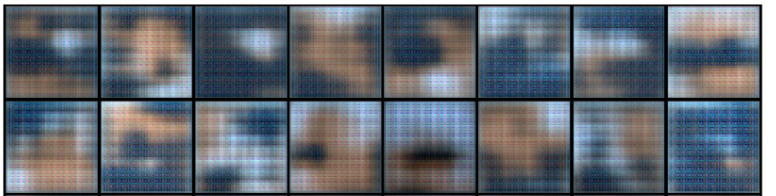
\includegraphics[scale=0.7]{../assets/model-1-1}
\end{center}

\underline{Epoch \# 2}
\begin{center}
	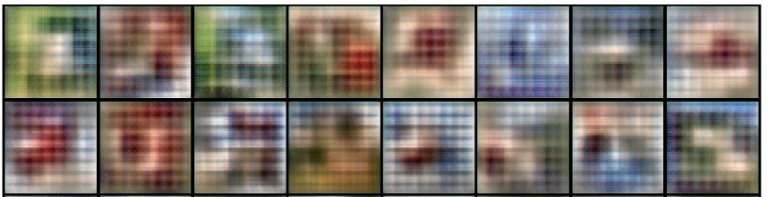
\includegraphics[scale=0.7]{../assets/model-1-2}
\end{center}


\underline{Epoch \# 80}
\begin{center}
	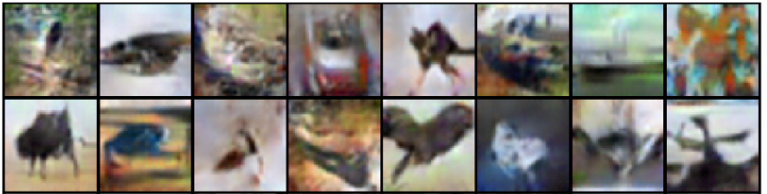
\includegraphics[scale=0.7]{../assets/model-1-3}
\end{center}

\pagebreak

(ii) \textbf{\textit{Learning rate = 0.0005}}\\

The model seemed to perform relatively well in this case. The results were analyzed at epochs 1, 2 and 15. The results were better even at the 15th epoch.
\begin{center}
	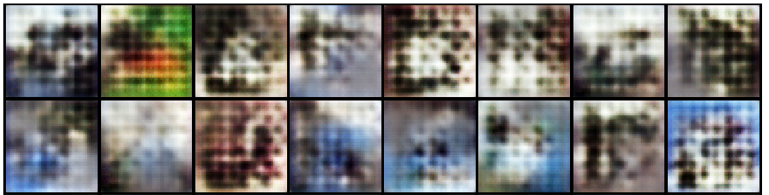
\includegraphics[scale=0.7]{../assets/model-2-1}
\end{center}

\underline{Epoch \# 2}
\begin{center}
	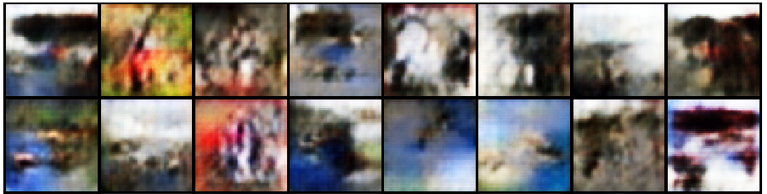
\includegraphics[scale=0.7]{../assets/model-2-2}
\end{center}


\underline{Epoch \# 15}
\begin{center}
	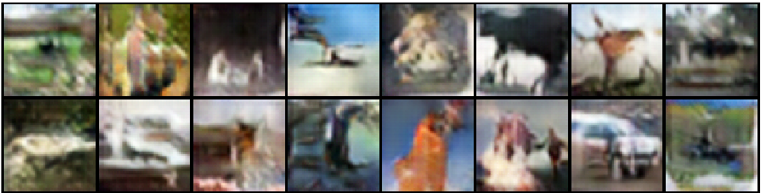
\includegraphics[scale=0.7]{../assets/model-2-3}
\end{center}

\pagebreak

(iii) \textbf{\textit{Learning rate = 0.0002}}\\

So far, 0.0002 learning rate performed the best among the three.

\begin{center}
	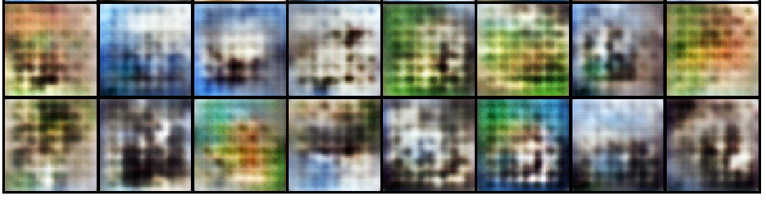
\includegraphics[scale=0.7]{../assets/model-3-1}
\end{center}

\underline{Epoch \# 2}
\begin{center}
	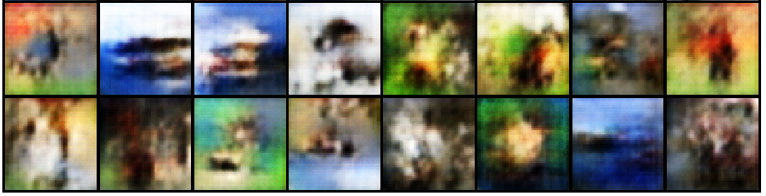
\includegraphics[scale=0.7]{../assets/model-3-2}
\end{center}


\underline{Epoch \# 15}
\begin{center}
	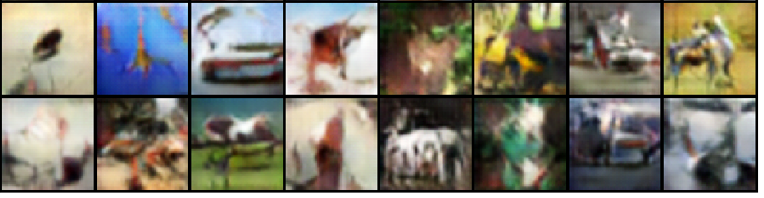
\includegraphics[scale=0.7]{../assets/model-3-3}
\end{center}

Among all the three models, model 3 performed the best even at 15 epochs. The loss was continuously decreasing and it can be said that if the same model is allowed to run for further epochs, it can generate even better results. 

\end{document}